%%%%%%%%%%%%%%%%%%%%%%%%%%%%%%%%%%%%%%%%%%%%%%%%%%%%%%%%%%%%%%
% CHAPTER 4
%%%%%%%%%%%%%%%%%%%%%%%%%%%%%%%%%%%%%%%%%%%%%%%%%%%%%%%%%%%%%%

\chapter{Data Preparation}

\section{Introduction}

Raw textual data collected from various sources often contains inconsistencies, noise, redundant information, and formatting variations that may adversely affect the performance of Natural Language Processing (NLP) models. Data preparation is therefore an essential step in the NLP pipeline to improve data quality and ensure compatibility with feature extraction and machine learning algorithms.

The preprocessing techniques selected for this project are based on the requirements of the Legal/Financial document classification and key-information-extraction tasks and the characteristics of the Hindi-language dataset described in Chapter 3. Only the preprocessing operations applicable to the selected task are performed. Each preprocessing step is justified based on its contribution to improving model performance.

%%%%%%%%%%%%%%%%%%%%%%%%%%%%%%%%%%%%%%%%%%%%%%%%%%%%%%%%%%%%%%

\section{Data Cleaning}

Data cleaning aims to remove unwanted information while preserving the semantic meaning of the text. As shown in Chapter 3, the raw dataset already contains no missing values, no duplicate records, and no HTML tags, emojis, or URLs (it is a clean, template-generated corpus of well-formed Hindi sentences). The cleaning operations below were therefore evaluated and applied selectively, only where relevant.

\newpage
\renewcommand{\arraystretch}{1.5}

\begin{longtable}{|p{5cm}|p{3cm}|p{7cm}|}
\caption{Data Cleaning Operations}
\label{tab:cleaning}\\

\hline
\textbf{Operation} &
\textbf{Applied (Yes/No)} &
\textbf{Justification}
\\
\hline
\endfirsthead

\hline
\textbf{Operation} &
\textbf{Applied (Yes/No)} &
\textbf{Justification}
\\
\hline
\endhead

Remove Duplicate Records & No (none found) & Verified in Chapter 3; 0 duplicate \texttt{Text} entries exist. \\ \hline

Remove Null Values & No (none found) & Verified in Chapter 3; 0 missing values across all columns. \\ \hline

Remove URLs & No & Legal/financial document text does not contain URLs. \\ \hline

Remove HTML Tags & No & Dataset is plain text, not scraped from web markup. \\ \hline

Remove Emojis & No & Formal legal/financial text does not contain emojis. \\ \hline

Remove Punctuation & Partial & Devanagari full stop (।) and standard punctuation are retained, as they carry sentence-boundary information needed for translation and QA; only extraneous symbols would be stripped. \\ \hline

Remove Special Characters & No & The currency symbol (₹) and \% sign are financially meaningful and are retained for key information extraction. \\ \hline

Remove Numbers & No & Dates, amounts, durations, and case numbers are critical extraction targets and must be preserved. \\ \hline

Unicode Normalization & Yes & Applied (NFC normalization) to ensure consistent encoding of Devanagari conjuncts and matras across all records. \\ \hline

Case Conversion & Not applicable & Devanagari script has no case distinction. \\ \hline

Whitespace Normalization & Yes & Extra/leading/trailing whitespace is normalized to ensure consistent tokenization. \\ \hline

Language-specific Cleaning & Yes & Normalization of Devanagari punctuation (।) usage for consistent sentence segmentation. \\ \hline

\end{longtable}

%%%%%%%%%%%%%%%%%%%%%%%%%%%%%%%%%%%%%%%%%%%%%%%%%%%%%%%%%%%%%%

\section{Tokenization}

Tokenization divides text into meaningful units for further processing. For Hindi, whitespace-based word tokenization is a reasonable first approximation since Devanagari text is space-delimited at the word level, but subword tokenization is preferred for transformer-based models to handle Hindi's morphological richness (inflections for gender, number, and case).

Possible techniques considered:

\begin{itemize}
\item Word Tokenization (whitespace-based)
\item Sentence Tokenization (Devanagari पूर्ण विराम ``।'' as delimiter)
\item Subword Tokenization
\item WordPiece (used internally by BERT/MuRIL-family models)
\item SentencePiece (used internally by IndicTrans2)
\end{itemize}

For exploratory analysis in this chapter, whitespace-based word tokenization is used (yielding a vocabulary of 1,196 unique tokens, as reported in Chapter 3). For the eventual classification and QA models, the WordPiece/SentencePiece tokenizer bundled with the selected pretrained model (MuRIL/IndicTrans2) will be used instead, since sub-word tokenization better handles unseen inflected forms in Hindi.

\subsection*{Example}

\begin{table}[H]
\centering
\caption{Tokenization Example}

\begin{tabular}{|p{6cm}|p{8cm}|}

\hline

Original Sentence &
ऋण दस्तावेज़ के अनुसार भारतीय स्टेट बैंक ने अजय पाटिल को ₹564670 का ऋण 14/12/2025 को स्वीकृत किया।
\\

\hline

Tokenized Output &
[ऋण, दस्तावेज़, के, अनुसार, भारतीय, स्टेट, बैंक, ने, अजय, पाटिल, को, ₹564670, का, ऋण, 14/12/2025, को, स्वीकृत, किया।]
\\

\hline

\end{tabular}

\end{table}

%%%%%%%%%%%%%%%%%%%%%%%%%%%%%%%%%%%%%%%%%%%%%%%%%%%%%%%%%%%%%%

\section{Stopword Processing}

Common Hindi function words such as \textit{की, के, का, को, में, है, ने, तथा} dominate the token-frequency list (Section~4.5.4). Whether these should be removed depends on the downstream task:

\begin{itemize}
\item For \textbf{document/intent classification} using TF-IDF or classical ML models, removing high-frequency stopwords can help the model focus on discriminative content words (e.g., ऋण, बीमा, न्यायालय, अनुबंध).
\item For \textbf{transformer-based classification and question answering}, stopwords are \textbf{retained}, since contextual models such as MuRIL rely on complete sentence structure -- and stopwords are essential for phrasing questions and answers naturally in Hindi.
\end{itemize}

Since the proposed pipeline (Chapter 5) uses a fine-tuned transformer for both classification and QA, stopwords are retained for the primary pipeline; stopword removal is treated as an optional preprocessing branch for classical ML baseline comparisons only.

\renewcommand{\arraystretch}{1.5}

\begin{table}[H]
\centering
\caption{Stopword Processing}

\begin{tabular}{|p{6cm}|p{8cm}|}

\hline

Stopwords Removed &
No (retained for transformer-based pipeline); optional for classical ML baselines
\\

\hline

Stopword Source &
Indic NLP Library Hindi stopword list (for the optional classical-ML branch)
\\

\hline

Reason &
Contextual transformer models require complete sentence structure; stopwords carry grammatical information needed for QA and translation.
\\

\hline

\end{tabular}

\end{table}

%%%%%%%%%%%%%%%%%%%%%%%%%%%%%%%%%%%%%%%%%%%%%%%%%%%%%%%%%%%%%%

\section{Morphological Processing}

Hindi is a morphologically rich, inflected language (verbs and nouns inflect for gender, number, case, and tense), so aggressive English-style stemming is not directly applicable.

Possible techniques include:

\begin{itemize}
\item Stemming
\item Lemmatization
\end{itemize}

Possible algorithms/tools:

\begin{itemize}
\item Indic NLP Library (rule-based Hindi stemmer)
\item iNLTK
\item Stanza (with Hindi UD models, for lemmatization)
\end{itemize}

\subsection*{Selected Technique}

Light rule-based Hindi \textbf{stemming} using the Indic NLP Library, applied only for the optional classical ML baseline (TF-IDF + Logistic Regression/SVM). No stemming is applied before transformer-based fine-tuning, since sub-word tokenizers (WordPiece/SentencePiece) already learn morphological regularities directly from data.

\subsection*{Justification}

Since the final proposed model (Chapter 5) is a fine-tuned transformer, morphological normalization is delegated to the sub-word tokenizer rather than applied manually. Manual stemming is retained only as a preprocessing option for lightweight classical ML baselines used for comparison.

\subsection*{Before and After Example}

\begin{table}[H]
\centering
\caption{Before and After Data Preprocessing Examples}
\label{tab:beforeafter}

\renewcommand{\arraystretch}{1.5}

\begin{tabular}{|p{4cm}|p{5.5cm}|p{5.5cm}|}
\hline
\textbf{Preprocessing Technique} &
\textbf{Before} &
\textbf{After}
\\
\hline

Whitespace Normalization &
"अनुबंध  की  अवधि" &
"अनुबंध की अवधि"
\\
\hline

Case Conversion &
Not applicable (Devanagari) &
Not applicable (Devanagari)
\\
\hline

Punctuation Retained &
कर्मचारी को ₹31717 मासिक पारिश्रमिक दिया जाएगा। &
कर्मचारी को ₹31717 मासिक पारिश्रमिक दिया जाएगा। (। retained as sentence boundary marker)
\\
\hline

Word Tokenization &
अनुबंध की अवधि 29 माह निर्धारित की गई है। &
[अनुबंध, की, अवधि, 29, माह, निर्धारित, की, गई, है।]
\\
\hline

Stopword Removal (optional ML branch) &
अनुबंध की अवधि 29 माह निर्धारित की गई है। &
अनुबंध अवधि 29 माह निर्धारित
\\
\hline

\end{tabular}

\end{table}

%%%%%%%%%%%%%%%%%%%%%%%%%%%%%%%%%%%%%%%%%%%%%%%%%%%%%%%%%%%%%%

\section{Exploratory Data Analysis (EDA)}

The following analyses, applicable to the DocSaarthi dataset, were performed directly on \texttt{DocSaarthi\_Dataset.csv}.

\begin{itemize}

\item Missing Value Analysis

\item Class Distribution (Document\_Type and Intent)

\item Vocabulary Size Analysis

\item Sentence Length Distribution

\item Most Frequent Tokens

\item N-gram (Bigram) Analysis

\item Word Cloud

\end{itemize}

%%%%%%%%%%%%%%%%%%%%%%%%%%%%%%%%%%%%%%%%%%%%%%%%%%%%%%%%%%%%%%

\subsection{Missing Value Analysis}

Table~\ref{tab:missing_values} presents the missing value analysis of the dataset. It can be observed that all four columns contain zero missing values, indicating that the dataset is complete and does not require any imputation before preprocessing.

\begin{table}[H]
\centering
\caption{Missing Value Analysis}
\label{tab:missing_values}
\begin{tabular}{|l|c|c|}
\hline
\textbf{Column Name} & \textbf{Missing Values} & \textbf{Percentage (\%)} \\
\hline
ID & 0 & 0.00 \\
Text & 0 & 0.00 \\
Document\_Type & 0 & 0.00 \\
Intent & 0 & 0.00 \\
\hline
\end{tabular}
\end{table}

\textbf{Observation:}
The dataset is complete, with no null values present in any column. Therefore, no missing value imputation was required before applying the NLP preprocessing pipeline.
%%%%%%%%%%%%%%%%%%%%%%%%%%%%%%%%%%%%%%%%%%%%%%%%%%%%%%%%%%%%%%

\subsection{Class Distribution}

Figure~\ref{fig:classdist} shows the distribution of the \texttt{Document\_Type} and \texttt{Intent} labels.

\begin{figure}[H]
\centering
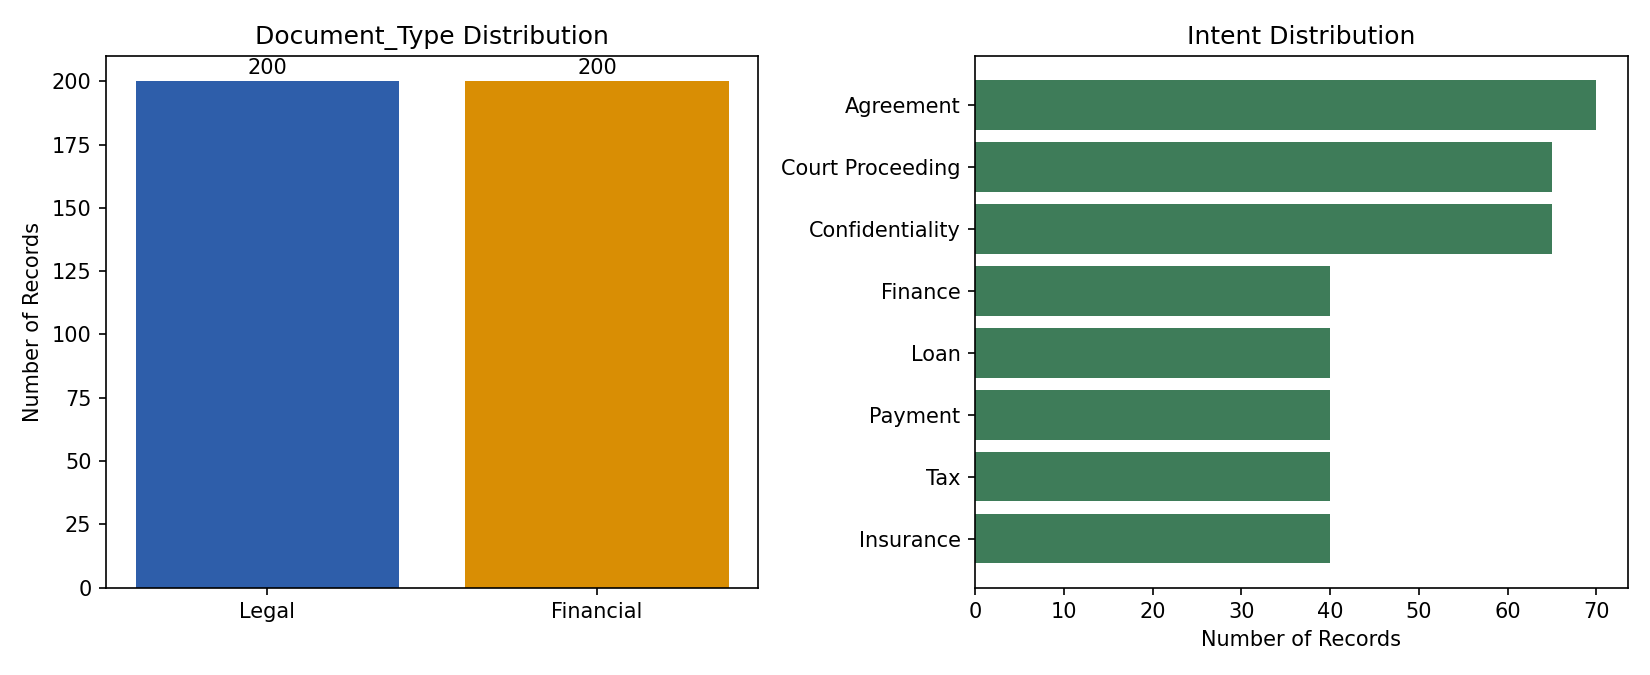
\includegraphics[width=0.95\textwidth]{figures/class_distribution.png}
\caption{Document\_Type and Intent Class Distribution}
\label{fig:classdist}
\end{figure}

\textbf{Observation:} \texttt{Document\_Type} is perfectly balanced (200 Legal / 200 Financial). \texttt{Intent} is moderately imbalanced: Agreement (70), Court Proceeding (65), and Confidentiality (65) are more frequent than the four Financial intents (40 each), reflecting the template-generation design. This imbalance should be accounted for (e.g., via class-weighted loss) when training the Intent classifier.

%%%%%%%%%%%%%%%%%%%%%%%%%%%%%%%%%%%%%%%%%%%%%%%%%%%%%%%%%%%%%%

\subsection{Vocabulary Analysis}

The dataset contains \textbf{1,196 unique whitespace-delimited tokens} across 400 records, giving a type-token ratio of approximately 1,196 / 18,764 $\approx$ 0.064, indicating a fairly repetitive, template-driven vocabulary -- expected given the synthetic generation process described in Chapter 3.

%%%%%%%%%%%%%%%%%%%%%%%%%%%%%%%%%%%%%%%%%%%%%%%%%%%%%%%%%%%%%%

\subsection{Sentence Length Distribution}

Figure~\ref{fig:sentlen} shows the histogram of record lengths measured in words.

\begin{figure}[H]
\centering
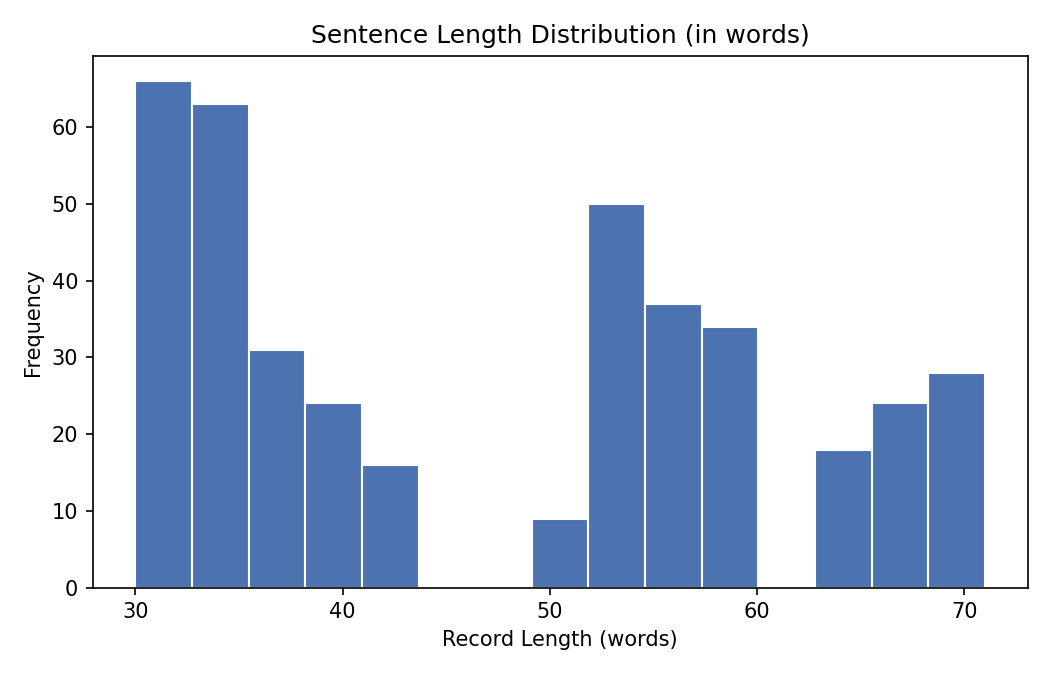
\includegraphics[width=0.75\textwidth]{figures/sentence_length_distribution.png}
\caption{Sentence Length Distribution (words per record)}
\label{fig:sentlen}
\end{figure}

\textbf{Observation:} Record lengths range from 30 to 71 words, with a mean of 46.9 words and a roughly bimodal spread reflecting the two document categories (shorter Financial notices versus longer Legal clauses). This length range is well within the input limits of standard transformer models (512 tokens), so no truncation is required.

%%%%%%%%%%%%%%%%%%%%%%%%%%%%%%%%%%%%%%%%%%%%%%%%%%%%%%%%%%%%%%

\subsection{Most Frequent Tokens}

Figure~\ref{fig:topfreq} shows the twenty most frequent tokens in the dataset.

\begin{figure}[H]
\centering
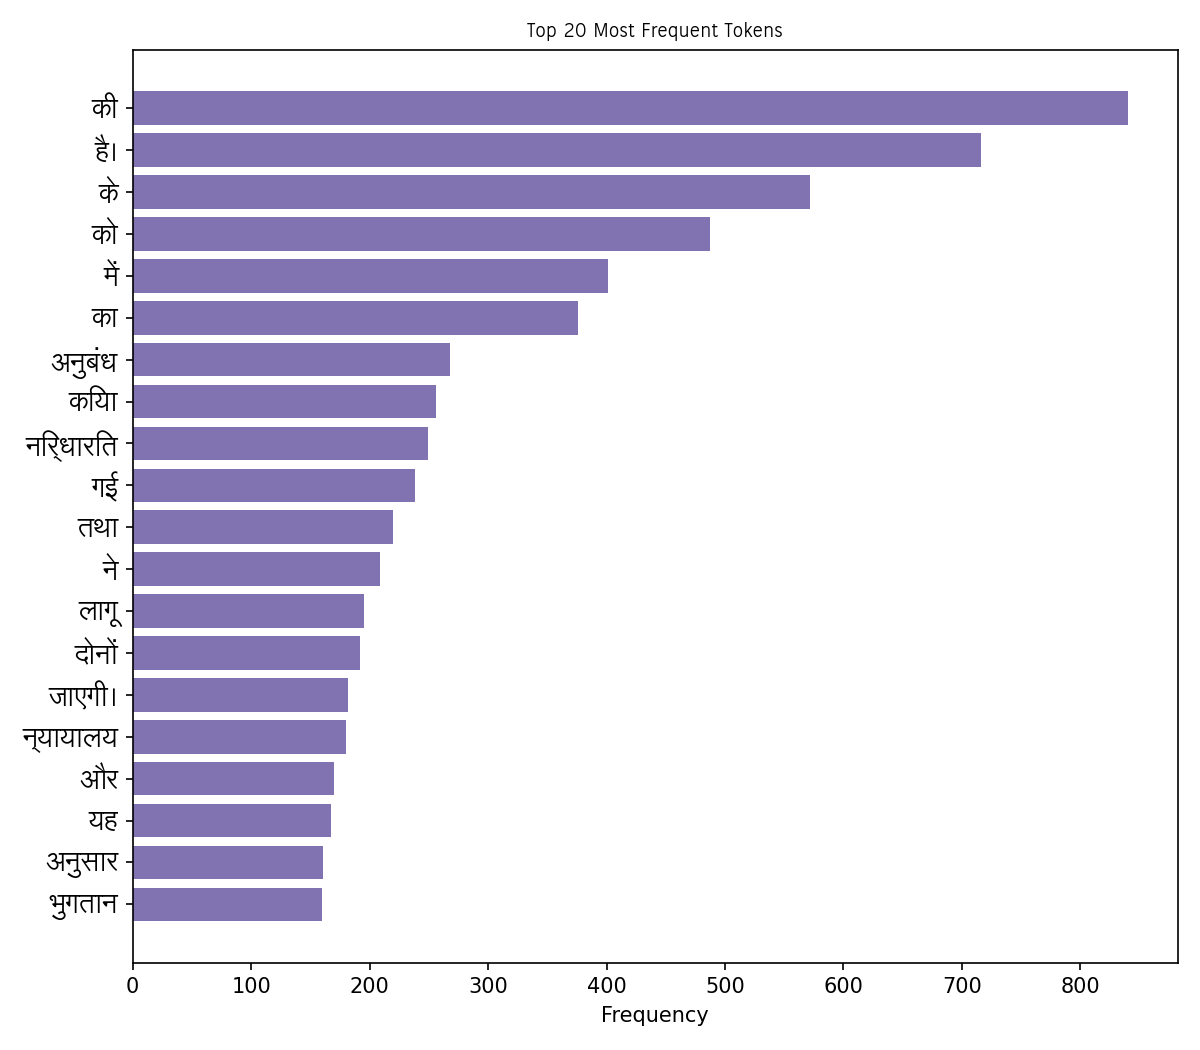
\includegraphics[width=0.7\textwidth]{figures/most_frequent_tokens.png}
\caption{Top 20 Most Frequent Tokens}
\label{fig:topfreq}
\end{figure}

\textbf{Observation:} The most frequent tokens (की, है।, के, को, में, का) are Hindi function words (postpositions and copulas), as expected. Content-bearing domain tokens such as अनुबंध (agreement/contract), निर्धारित (fixed/determined), न्यायालय (court), and भुगतान (payment) also appear among the top 20, confirming that the dataset carries clear domain signal beyond generic function words.

%%%%%%%%%%%%%%%%%%%%%%%%%%%%%%%%%%%%%%%%%%%%%%%%%%%%%%%%%%%%%%

\subsection{N-gram Analysis}

Table~\ref{tab:bigrams} presents the ten most frequent bigrams found in the dataset.

\begin{table}[H]
\centering
\caption{Top 10 Most Frequent Bigrams}
\label{tab:bigrams}
\begin{tabular}{|p{6cm}|p{3cm}|}
\hline
\textbf{Bigram} & \textbf{Frequency} \\
\hline
गई है। & 221 \\ \hline
निर्धारित की & 215 \\ \hline
की गई & 215 \\ \hline
के अनुसार & 161 \\ \hline
की जाएगी। & 156 \\ \hline
किया गया। & 136 \\ \hline
के बीच & 135 \\ \hline
दोनों पक्षों & 122 \\ \hline
किया गया & 112 \\ \hline
गया है। & 112 \\ \hline
\end{tabular}
\end{table}

\textbf{Observation:} The dominant bigrams (``निर्धारित की'', ``की गई'', ``के अनुसार'') are formal legal/financial phrasing patterns (``...is determined'', ``...as per...''), confirming the formulaic, clause-based writing style typical of legal and financial documents.

%%%%%%%%%%%%%%%%%%%%%%%%%%%%%%%%%%%%%%%%%%%%%%%%%%%%%%%%%%%%%%

\subsection{Word Cloud}

Figure~\ref{fig:wordcloud} presents a word cloud generated from the complete dataset vocabulary.

\begin{figure}[H]
\centering
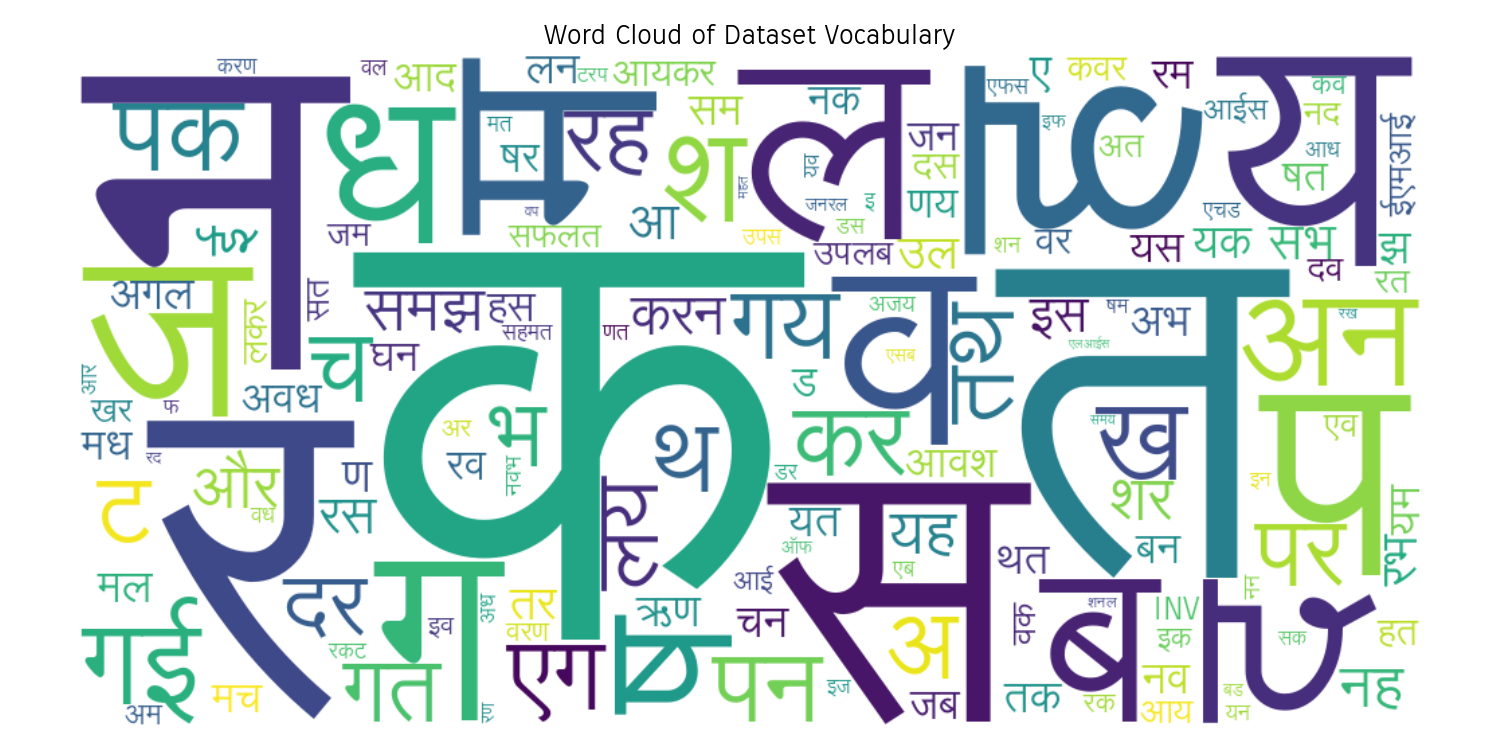
\includegraphics[width=0.85\textwidth]{figures/wordcloud.png}
\caption{Word Cloud of Dataset Vocabulary}
\label{fig:wordcloud}
\end{figure}

\textbf{Observation:} The word cloud visually reinforces the frequency analysis, with domain terms such as अनुबंध, न्यायालय, भुगतान, and निर्धारित appearing prominently alongside common Hindi function words.

%%%%%%%%%%%%%%%%%%%%%%%%%%%%%%%%%%%%%%%%%%%%%%%%%%%%%%%%%%%%%%

\subsection{Other Applicable Analyses}

Character-level and language distribution analyses were reported in Table~3.5 (Chapter 3): the dataset is 100\% Devanagari-script Hindi text with an average record length of 262 characters, and required no out-of-vocabulary (OOV) analysis since it is a closed, self-generated corpus.

%%%%%%%%%%%%%%%%%%%%%%%%%%%%%%%%%%%%%%%%%%%%%%%%%%%%%%%%%%%%%%

\section{Preprocessing Workflow}

Figure~\ref{fig:preprocessingworkflow} illustrates the complete preprocessing pipeline used in the proposed project.

\begin{figure}[H]

\centering

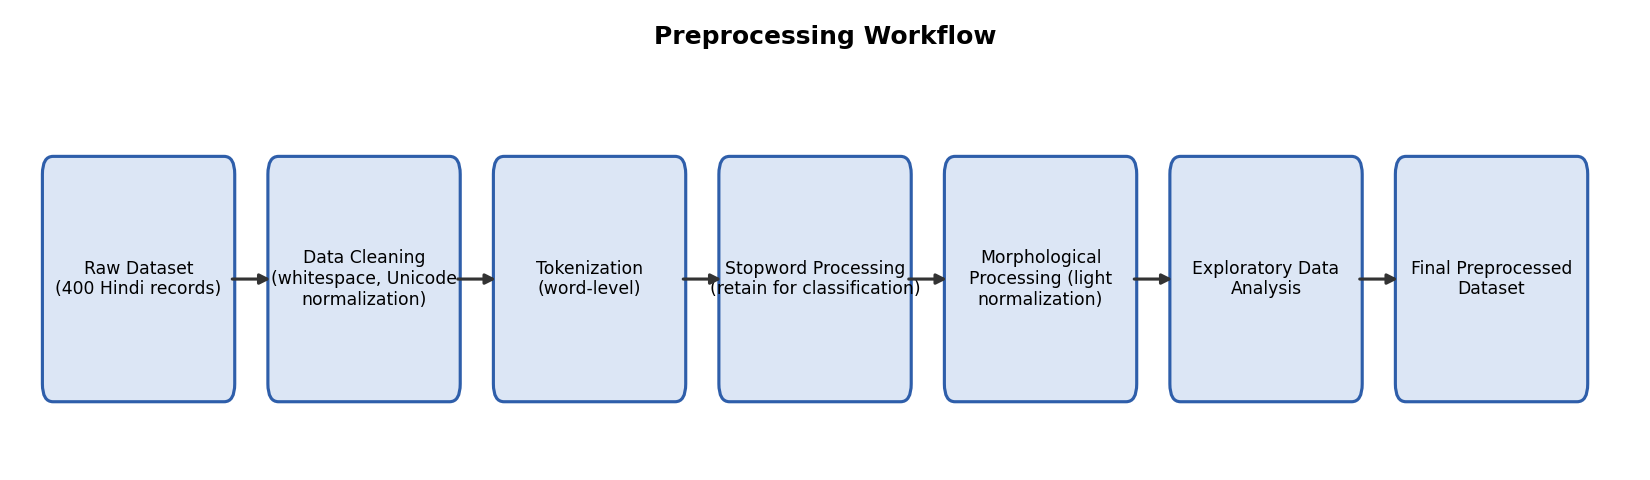
\includegraphics[width=0.95\textwidth]{figures/preprocessing_workflow.png}

\caption{Preprocessing Workflow}

\label{fig:preprocessingworkflow}

\end{figure}

The workflow illustrates:

\begin{itemize}

\item Raw Dataset (400 Hindi legal/financial records)

\item Data Cleaning (Unicode and whitespace normalization)

\item Tokenization (word-level for EDA; sub-word for model input)

\item Stopword Processing (retained for transformer pipeline; optional removal for classical ML baseline)

\item Morphological Processing (delegated to sub-word tokenizer; optional stemming for baseline)

\item Exploratory Data Analysis (class distribution, vocabulary, sentence length, n-grams)

\item Final Preprocessed Dataset (ready for feature representation and model training, Chapter 5)

\end{itemize}

\section{Preprocessing Implementation}

The implemented Node.js pipeline normalizes Unicode text, repairs whitespace and PDF line-break artefacts, preserves Devanagari combining marks, divides pages into evidence chunks, and retains each chunk's page number. Stopwords are not removed from the source evidence because legal negation and function words can change meaning. Translation is deferred until requested so that document upload remains fast and independent of a translation service.

\section{Before and After Preprocessing Analysis}

\begin{table}[H]
\centering
\caption{Representative Before and After Preprocessing Cases}
\begin{tabular}{|p{5.8cm}|p{7.2cm}|}
\hline
\textbf{Before} & \textbf{After} \\
\hline
Repeated spaces and isolated PDF line breaks & Normalized spacing with sentence continuity restored \\
\hline
Mixed Unicode forms in Hindi text & Unicode-normalized Devanagari with combining marks preserved \\
\hline
Complete document treated as one search unit & Page-linked chunks suitable for focused retrieval \\
\hline
Translation coupled to upload & Original source stored first; translation performed only on demand \\
\hline
\end{tabular}
\end{table}

The analysis shows that preprocessing improves retrieval consistency without rewriting the authoritative source text. Numeric values, dates, percentages, names, and page references remain available for answer verification.

%%%%%%%%%%%%%%%%%%%%%%%%%%%%%%%%%%%%%%%%%%%%%%%%%%%%%%%%%%%%%%

\section*{Chapter Summary}

This chapter presented the preprocessing techniques applied to the DocSaarthi dataset before model development. Data cleaning confirmed the dataset was already free of missing values, duplicates, and noise; Unicode and whitespace normalization were nonetheless applied. Tokenization, stopword processing, and morphological processing were evaluated and selectively applied based on whether the downstream model is a transformer (stopwords/morphology retained, delegated to the sub-word tokenizer) or a classical ML baseline (stopwords/stemming applied). Exploratory data analysis revealed a perfectly balanced Document\_Type split, a moderately imbalanced Intent distribution, a compact 1,196-word vocabulary reflecting the dataset's template-driven generation, and clause-based bigram patterns typical of legal/financial writing. The resulting preprocessed dataset forms the input for the feature representation and model design discussed in the next chapter.
